\documentclass[a4paper, 11pt]{report}
\usepackage[utf8]{inputenc}
\usepackage{titlesec}
\usepackage{fullpage} % changes the margin
\usepackage{graphicx} %package to manage images
\graphicspath{ {./images/} }

\begin{document}
\begin{titlepage}
\vspace*{0.7in}
\begin{center}
\begin{figure}[htb]
\begin{center}

\includegraphics[width=8cm]{univ_logo}
\end{center}
\end{figure}
\vspace*{0.3in}
\begin{Large}
\textbf{SOEN 6011 : SOFTWARE ENGINEERING PROCESSES} \\
\end{Large}
\vspace*{0.1in}
\begin{Large}
\textbf{SUMMER 2021} \\
\end{Large}
\vspace*{0.9in}
\begin{Large}
\textbf{SUPER CALCULATOR} \\
\end{Large}
\vspace*{0.9in}
\begin{Large} 


\textbf{PROBLEM - 6} \\
Unit Test Cases\\
\end{Large}
\vspace*{0.9in}
\rule{80mm}{0.1mm}\\
\vspace*{0.1in}
\begin{large}
Authors \\
\vspace*{0.1in}
Rokeya Begum Keya\\
\vspace*{0.1in}
Kyle Taylor Lange\\
\vspace*{0.1in}
Sijie Min\\
\vspace*{0.1in}
Manimaran Palani\\ 
\vspace*{0.3in}
\date{\normalsize\today} 
\end{large}
\end{center}
\begin{center}
https://www.overleaf.com/project/610304de4e6b8d24f7c781b6\end{center}
\end{titlepage}
\tableofcontents
\newpage
\addcontentsline{toc}{section}{a) Description on Unit Test Cases }
\newpage
\pagebreak
\section*{Unit Test Cases Description}
\section*{\centering{PROBLEM 6 - F2: $tan(x)$}}
\normalsize {SOEN 6011 - Summer 2021} \hfill \textbf{Rokeya Begum Keya} \\
\textbf{ Software Engineering Processes}  \hfill \textbf{40183615} \\
\hfill Repository address : https://github.com/Dakatsu/SOEN6011Calculator
\\\\\\

\pagebreak

\section*{\centering{PROBLEM 6 - F3: Hyperbolic Sine, $sinh(x)$}}
\normalsize {SOEN 6011 - Summer 2021} \hfill \textbf{Kyle Taylor Lange} \\
\textbf{ Software Engineering Processes}  \hfill \textbf{27627696} \\https://www.overleaf.com/project/610304de4e6b8d24f7c781b6
\hfill Repository address : https://github.com/Dakatsu/SOEN6011Calculator
\\\\\\

\pagebreak

\section*{\centering{PROBLEM 6 - F5}}
\normalsize {SOEN 6011 - Summer 2021} \hfill \textbf{Sijie Min} \\
\textbf{ Software Engineering Processes}  \hfill \textbf{401*****} \\
\hfill Repository address : https://github.com/Dakatsu/SOEN6011Calculator
\\\\\\\\\\
 \begin{center} Team please add your content here \end{center}
\pagebreak

\section*{\centering{PROBLEM 6 - F7 : \(x^y\)}}
\normalsize {SOEN 6011 - Summer 2021} \hfill \textbf{Manimaran Palani} \\
\textbf{ Software Engineering Processes}  \hfill \textbf{40167543} \\
\hfill Repository address : https://github.com/Dakatsu/SOEN6011Calculator
\\
\section*{\textbf{Problem 6 - Unit Test Case Description}}
This section presents the unit test cases implemented using \textbf{JUnit4} for Super Calculator \\(F7-Power Function) which are traceable to requirements.\\\\\\
\textbf{Test Case : F7\_TestCase\_1}\\\\
\begin{tabular}{ll}
\textbf{Test Case ID} & F7\_TestCase\_1 \\
\textbf{Requirement ID} & F7-R1 \\
\textbf{Action} & 
\begin{tabular}[c]{@{}l@{}}The user inputs a base input and click power function button followed \\by giving exponent input and click result(=) button. \\
\end{tabular} \\
\textbf{Input(s) } & base = 0.0, exponent = 0.0 \\
\textbf{Expected Output } & 1.0 \\
\textbf{Actual Output } & 1.0 \\
\textbf{Test Result } & Success \\
\end{tabular}
\\\\\\\\
\textbf{Test Case : F7\_TestCase\_2}\\\\
\begin{tabular}{ll}
\textbf{Test Case ID} & F7\_TestCase\_2 \\
\textbf{Requirement ID} & F7-R2 \\
\textbf{Action} & 
\begin{tabular}[c]{@{}l@{}}The user inputs a base input and click power function button followed \\by giving exponent input and click result(=) button. \\
\end{tabular} \\
\textbf{Input(s) } & base = 0.0, exponent = 3.0 \\
\textbf{Expected Output } & 0.0 \\
\textbf{Actual Output } & 0.0 \\
\textbf{Test Result } & Success \\
\end{tabular}
\\\\\\\\
\textbf{Test Case : F7\_TestCase\_3}\\\\
\begin{tabular}{ll}
\textbf{Test Case ID} & F7\_TestCase\_3 \\
\textbf{Requirement ID} & F7-R3 \\
\textbf{Action} & 
\begin{tabular}[c]{@{}l@{}}The user inputs a base input and click power function button followed \\by giving exponent input and click result(=) button. \\
\end{tabular} \\
\textbf{Input(s) } & base = 7.0, exponent = 0.0 \\
\textbf{Expected Output } & 1.0 \\
\textbf{Actual Output } & 1.0 \\
\textbf{Test Result } & Success \\
\end{tabular}
\\\\\\\\
\textbf{Test Case : F7\_TestCase\_4}\\\\
\begin{tabular}{ll}
\textbf{Test Case ID} & F7\_TestCase\_4 \\
\textbf{Requirement ID} & F7-R4 \\
\textbf{Action} & 
\begin{tabular}[c]{@{}l@{}}The user inputs a base input and click power function button followed \\by giving exponent input and click result(=) button. \\
\end{tabular} \\
\textbf{Input(s) } & base = -4.0, exponent = 0.0 \\
\textbf{Expected Output } & 1.0 \\
\textbf{Actual Output } & 1.0 \\
\textbf{Test Result } & Success \\
\end{tabular}
\\\\\\\\
\textbf{Test Case : F7\_TestCase\_5}\\\\
\begin{tabular}{ll}
\textbf{Test Case ID} & F7\_TestCase\_5 \\
\textbf{Requirement ID} & F7-R5 \\
\textbf{Action} & 
\begin{tabular}[c]{@{}l@{}}The user inputs a base input and click power function button followed \\by giving exponent input and click result(=) button. \\
\end{tabular} \\
\textbf{Input(s) } & base = 7.0, exponent = 1.0 \\
\textbf{Expected Output } & 7.0 \\
\textbf{Actual Output } & 7.0 \\
\textbf{Test Result } & Success \\
\end{tabular}
\\\\\\\\
\textbf{Test Case : F7\_TestCase\_6}\\\\
\begin{tabular}{ll}
\textbf{Test Case ID} & F7\_TestCase\_6 \\
\textbf{Requirement ID} & F7-R6 \\
\textbf{Action} & 
\begin{tabular}[c]{@{}l@{}}The user inputs a base input and click power function button followed \\by giving exponent input and click result(=) button. \\
\end{tabular} \\
\textbf{Input(s) } & base = 5, exponent = 9 \\
\textbf{Expected Output } & 1953125.0 \\
\textbf{Actual Output } & 1953125.0 \\
\textbf{Test Result } & Success \\
\end{tabular}
\\\\\\\\
\textbf{Test Case : F7\_TestCase\_7}\\\\
\begin{tabular}{ll}
\textbf{Test Case ID} & F7\_TestCase\_7 \\
\textbf{Requirement ID} & F7-R6 \\
\textbf{Action} & 
\begin{tabular}[c]{@{}l@{}}The user inputs a base input and click power function button followed \\by giving exponent input and click result(=) button. \\
\end{tabular} \\
\textbf{Input(s) } & base = -3, exponent = 4.4     \\
\textbf{Expected Output } & 3.1631 \\
\textbf{Actual Output } & 3.1631 \\
\textbf{Test Result } & Success \\
\end{tabular}
\\\\\\\\
\textbf{Test Case : F7\_TestCase\_8}\\\\
\begin{tabular}{ll}
\textbf{Test Case ID} & F7\_TestCase\_8 \\
\textbf{Requirement ID} & F7-R6 \\
\textbf{Action} & 
\begin{tabular}[c]{@{}l@{}}The user inputs a base input and click power function button followed \\by giving exponent input and click result(=) button. \\
\end{tabular} \\
\textbf{Input(s) } & base = -9, exponent = 3 \\
\textbf{Expected Output } & -729 \\
\textbf{Actual Output } & -729 \\
\textbf{Test Result } & Success \\
\end{tabular}\\\\\\\\
\textbf{Test Case Results for F7}
\begin{figure}[htb]
\begin{center}
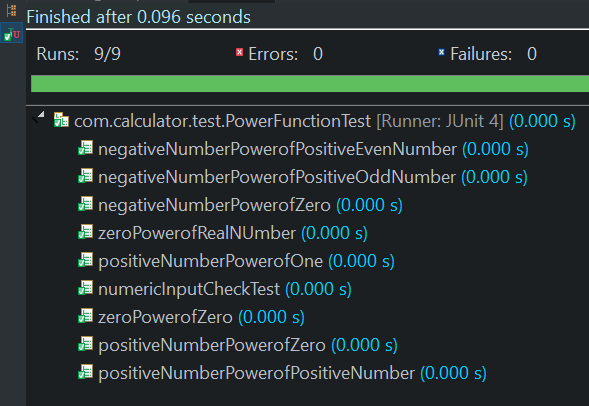
\includegraphics[width=13cm]{TestCases_Results_F7}
  \centering
  \caption{ Test case result of function F7 : \(x^y\)  using Junit4
}
\end{center}
\end{figure}
\end{document}